\documentclass[10pt,letterpaper]{article}
\usepackage[utf8]{inputenc}
\usepackage[T1]{fontenc}
\usepackage{lmodern}
\usepackage{microtype}
\usepackage[margin=0.48in,top=0.52in,bottom=0.52in]{geometry}
\usepackage{amsmath,amssymb,amsfonts}
\usepackage{booktabs}
\usepackage{tabularx}
\usepackage{array}
\usepackage{placeins}
\usepackage{xcolor}
\PassOptionsToPackage{hyphens}{url}
\usepackage{hyperref}
\def\UrlBreaks{\do\/\do-\do_\do.\do:\do0\do1\do2\do3\do4\do5\do6\do7\do8\do9\do a\do b\do c\do d\do e\do f}
\usepackage{enumitem}
\usepackage{tikz}
\usetikzlibrary{arrows.meta,positioning,shapes.geometric,calc}
\usepackage{fancyhdr}
\usepackage{titlesec}
\usepackage{etoolbox}

\definecolor{navy}{HTML}{0F2C59}
\definecolor{slate}{HTML}{334155}
\definecolor{accent}{HTML}{1D4ED8}
\definecolor{boxbg}{HTML}{F8FAFC}
\definecolor{boxborder}{HTML}{CBD5E1}
\definecolor{goodgreen}{HTML}{15803D}
\definecolor{warnamber}{HTML}{B45309}
\definecolor{badred}{HTML}{B91C1C}

\hypersetup{
    colorlinks=true,
    linkcolor=accent,
    citecolor=accent,
    urlcolor=accent,
    pdftitle={EmbodiedX Real-Time Embodied AI Inference Benchmark Methodology and Specification (v1.0.0)},
    pdfauthor={CoRL 2026 EEAI Workshop Organizing Committee}
}

\pagestyle{fancy}
\fancyhf{}
\fancyhead[L]{\footnotesize\textcolor{slate}{\textbf{EmbodiedX v1.0.0} Real-Time Embodied AI Inference Benchmark (CoRL 2026 EEAI Workshop)}}
\fancyhead[R]{\footnotesize\textcolor{slate}{Methodology Specification}}
\fancyfoot[C]{\footnotesize\thepage}
\renewcommand{\headrulewidth}{0.4pt}
\setlength{\headheight}{13pt}

\titleformat{\section}{\large\bfseries\color{navy}}{\thesection.}{0.45em}{}[\titlerule]
\titleformat{\subsection}{\normalsize\bfseries\color{navy}}{\thesubsection}{0.45em}{}
\titleformat{\subsubsection}{\normalsize\bfseries\color{slate}}{\thesubsubsection}{0.45em}{}
\titlespacing*{\section}{0pt}{0.50em}{0.18em}
\titlespacing*{\subsection}{0pt}{0.36em}{0.12em}
\titlespacing*{\subsubsection}{0pt}{0.28em}{0.08em}

\setlength{\parskip}{0.14em}
\setlength{\parindent}{0pt}
\emergencystretch=3em
\setlist[itemize]{leftmargin=1.4em, itemsep=0.06em, topsep=0.05em}
\setlist[enumerate]{leftmargin=1.5em, itemsep=0.06em, topsep=0.05em}

\patchcmd{\thebibliography}{\usecounter{enumiv}}{\usecounter{enumiv}\setlength{\itemsep}{1.5pt}\setlength{\parsep}{0pt}\setlength{\parskip}{0pt}}{}{}

\newcommand{\cmark}{\textcolor{goodgreen}{\textbf{Yes}}}
\newcommand{\wmark}{\textcolor{warnamber}{\textbf{Partial}}}
\newcommand{\xmark}{\textcolor{badred}{\textbf{No}}}

\begin{document}
\nocite{Patel2025inferencemax,Patel2026inferencexv2,Patel2026agentx,Zhao2023learning,Chi2024diffusion,Black2024pi0,PhysicalIntelligence2025pi05,Bjorck2025gr00t,Kim2025finetuning,Black2025realtime,Liu2023libero,Li2024evaluating,Mees2022calvin,Stanford2026behavior,Ramstedt2019realtime,Xiao2020thinking,Tang2025vlash,Black2025trainingtime,Agouzoul2026understanding,AllenAI2026vlaeval,Kaul2012realtime,Costa2016age,Yates2021age,Shukor2025smolvla,NVIDIA2025cosmos,Qwen2025qwen3omni,Liao2025genie,Fei2025liberoplus,Zhang2025vlaarena,MLCommons2026power,Chung2025mlenergy,Luccioni2025aienergy,Yue2024deervla,Williams2009roofline,Reddi2020mlperf,Mereu2025generative,MayoralVilches2024robotperf,Yue2025ewmbench,Duan2025worldscore,Shang2026worldarena,Shang2026worldarena2,Xu2025vlacache,Yang2025efficientvla,Tan2025think,Wang2025specvla,Pertsch2025fast,Atreya2025roboarena,Yates2019age,Ramstedt2020reinforcement,Riemer2024enabling,Jiang2025streaming,Guan2025efficient,Yu2025survey,Zhang2025experiences,Sendai2025a2c2,Wang2025bitvla,Chen2025fisvla,Wen2024tinyvla,Chen2024diffusionforcing,Yin2025causvid,Huang2025selfforcing,Valevski2024gamengen,He2025matrixgame2,Xi2025sparsevideogen,Li2025radialattention,Zhou2024dinowm,Boroujerdian2018mavbench,Tao2024maniskill3}

\begin{center}
    {\LARGE\bfseries\color{navy} EmbodiedX Real-Time Embodied AI Inference Benchmark}\\[0.35em]
    {\normalsize\bfseries\color{slate} Methodology Specification and Literature Synthesis Across Single-Chip Cloud GPU and TPU Accelerators}\\[0.35em]
    {\small \textbf{CoRL 2026 Workshop on Efficient Foundation Models for Real-Time Embodied AI (EEAI)}\\
    Organizing Committee Specification Report (v1.0.0) $\cdot$ \texttt{efficient-embodied-ai/embodied-efficiency-bench} $\cdot$ \url{https://efficient-embodied-ai.github.io/challenge/}}
\end{center}
\vspace{0.2em}
\hrule
\vspace{0.4em}

\section{Motivation and Season 1 Design Summary}

Embodied AI foundation models span Vision-Language-Action (VLA) control policies ($\pi_0$ \cite{Black2024pi0}, $\pi_{0.5}$ \cite{PhysicalIntelligence2025pi05}, \texttt{GR00T N1 / N1.7-3B} \cite{Bjorck2025gr00t}, \texttt{SmolVLA} \cite{Shukor2025smolvla}) and action-conditioned world models (\texttt{Cosmos-Predict2.5-2B} \cite{NVIDIA2025cosmos}, \texttt{Genie Envisioner} \cite{Liao2025genie}). Recent inference work accelerates these models through custom device kernels (\texttt{Pallas}, \texttt{Triton}, \texttt{CUDA}), cross-frame visual token caching (\texttt{VLA-Cache} \cite{Xu2025vlacache}), numerical quantization and compression (\texttt{FP8}, \texttt{INT8}, \texttt{INT4}, \texttt{EfficientVLA} \cite{Yang2025efficientvla,Guan2025efficient,Yu2025survey}), and asynchronous action-chunk scheduling (\texttt{RTC} \cite{Black2025realtime}, \texttt{TT-RTC} \cite{Black2025trainingtime}, \texttt{VLASH} \cite{Tang2025vlash}).

Standard robotics leaderboards evaluate models in stop-and-wait simulators where physics pauses during neural inference. Under a frozen simulation clock, a $2{,}000\text{ ms}$ policy and a $20\text{ ms}$ policy experience identical zero actuation delay, which hides physical control failures caused by object slip or contact drift mid-trajectory. Meanwhile, modern ML serving benchmarks such as \textbf{SemiAnalysis InferenceX (InferenceMAX)} \cite{Patel2025inferencemax,Patel2026inferencexv2} and \textbf{MLPerf Inference} \cite{Reddi2020mlperf} plot \textbf{Throughput (\texttt{tok/s/chip}) vs.\ Interactivity (\texttt{tok/s/user})} Pareto frontiers for autoregressive token streaming, whose axes do not capture receding-horizon action chunking or closed-loop actuation deadlines.

\textbf{EmbodiedX (\texttt{embodied-efficiency-bench} v1.0.0)} defines an open-source closed-loop serving benchmark for the \textbf{CoRL 2026 EEAI Workshop}. Season 1 executes every submission on one physical chip (\texttt{num\_devices == 1}, $\text{TP} = \text{PP} = \text{EP} = 1$) across two standardized cloud platforms: \textbf{NVIDIA L40S (48 GB GDDR6)} and \textbf{Google Cloud TPU v6e-1 (32 GB HBM2e)}. Every evaluation trace is drawn deterministically from public real-world datasets (\texttt{HuggingFaceVLA/libero} and \texttt{lerobot/droid\_100}), with zero synthetic sine-wave traces permitted in submissions. Under Option A launch neutrality, Season 1 opens on October 30, 2026 with $0$ organizer-seeded vendor benchmark entries on the leaderboard so community pull requests establish the founding Pareto frontier directly.

\subsection{Ten Architectural Decisions for EmbodiedX v1.0.0}

EmbodiedX enforces ten architectural decisions (\textbf{D1--D10}, recorded in \texttt{docs/DESIGN\_DECISIONS.md}):
\begin{enumerate}
    \item \textbf{D1 (Closed and Open Divisions Under Locked $K_{\text{eval}}$ and Host-CPU Offload Ban).} Both \texttt{Closed} and \texttt{Open} divisions lock execution horizon $K_{\text{eval}}$ ($5$ actions on Track 1A, $8$ actions on Track 1B, $16$ predicted frames per rollout prediction on Track 2) so aggregate output cannot be inflated by lengthening open-loop horizons. Across both divisions, $100\%$ of neural forward-pass operators (\texttt{MatMul}, \texttt{Attention}, \texttt{Conv}, \texttt{MLP}, \texttt{VAE}, text encoders) inside timed \texttt{act()} and \texttt{rollout()} calls must execute on the single target accelerator; host CPU threads handle only I/O, tokenization, RPC dispatch, and action queuing, while constant episode prompt embeddings may be pre-cached on the target accelerator during untimed \texttt{reset()}. \textbf{Closed Division} keeps checkpoint architecture and pretrained weights fixed at reference solver step counts under BF16/FP16/FP8 numerics checked by inline Golden-IO parity ($\ge 100$ real trace samples with mean quality floors and $\text{CVaR-1\%}$ worst-tail floors) and forbids pseudo-causal sub-clip slicing (\texttt{stream\_chunk\_frames > 0}) on Track 2. \textbf{Open Division} permits INT4 quantization, pruning, step distillation, or token merging when paired with a signed Stage-2 quality receipt.
    \item \textbf{D2 (Three Independent Track Pools Anchored to Gapless Real-Time SLAs and Pinned Checkpoints).} At a $20\text{ Hz}$ servo loop ($\Delta t = 50\text{ ms}$, where $20.0\text{ Chunks/s}$ is the single-tick reaction ceiling), executing $K_{\text{eval}}$ steps covers $K_{\text{eval}}\Delta t$:
    \begin{itemize}
        \item \textbf{Track 1A (\texttt{pi0.5-LIBERO}).} Physical Intelligence $\pi_{0.5}$ \cite{PhysicalIntelligence2025pi05} loaded from canonical ungated checkpoint \path{lerobot/pi05_libero_finetuned_v044} (commit \path{7152f13e34c6c115d808aea0e5d08aca74eac14b}, with pre-fit normalizers; $10$ Euler ODE steps, dual $224\times 224$ RGB traces from \path{HuggingFaceVLA/libero} commit \path{86958911c0f959db2bbbdb107eb3e17c5f9c798e}, $H = 10$, locked $K_{\text{eval}} = 5$, $\approx 0.734\text{ TF/action}$), gapless SLA \textbf{$L_{p99} \le 250.0\text{ ms}$ ($\ge 4.0\text{ Chunks/s}$)}. Both \texttt{PyTorch} (\texttt{CUDA} / \texttt{TorchTPU}) and \texttt{openpi} \texttt{JAX} are certified reference runtimes.
        \item \textbf{Track 1B (\texttt{GR00T N1.7-3B}).} NVIDIA \texttt{GR00T N1.7-3B} \cite{Bjorck2025gr00t} loaded from \path{nvidia/GR00T-N1.7-LIBERO} (\texttt{libero\_10} subfolder, commit \path{2ea293aa20ba7cf5bbf3ba17a5fbcb1a01cbfe21}; \texttt{Cosmos-Reason2-2B} VLM + $16$-step DiT flow action head, dual $256\times 256$ RGB traces from \path{HuggingFaceVLA/libero}, $H = 16$, locked $K_{\text{eval}} = 8$, $\approx 0.404\text{ TF/action}$), gapless SLA \textbf{$L_{p99} \le 400.0\text{ ms}$ ($\ge 2.5\text{ Chunks/s}$)}. Track 1A and Track 1B maintain separate award pools because \texttt{GR00T N1.7-3B} executes $1.82\times$ fewer FLOPs per action than $\pi_{0.5}$.
        \item \textbf{Track 2 (\texttt{Cosmos-Predict2.5-2B}).} NVIDIA \texttt{Cosmos-Predict2.5-2B} \cite{NVIDIA2025cosmos} loaded from checkpoint \path{nvidia/Cosmos-Predict2.5-2B} (\path{robot/action-cond} action-conditioned weights, commit \path{85f8ae7bfe8f5525c8d103429524dcf12f98bf7b}; bidirectional 3D-DiT video world model, $10$ steps, $\text{CFG} = 1.0$, real-world $256\times 256$ RGB manipulation traces from \path{lerobot/droid_100} commit \path{87301a2d2e99340e2010c9ef0f1d8e780b08aaf9}, locked $K_{\text{eval}} = 16$ frames per rollout prediction), gapless SLA \textbf{$L_{p99,\text{WM}} \le 1000.0\text{ ms}$ ($\ge 1.0\text{ Pred/s}$)}.
    \end{itemize}
    \item \textbf{D3 (Quality Verification as a Hard Admissibility Gate).} Golden parity sets require \texttt{-{}-num-samples >= 100} real trace frames. In \texttt{Closed}, Track 1 enforces inline Golden-IO $\text{CosSim} \ge 0.995$ plus $\text{CVaR-1\%}$ floor, and Track 2 enforces $\text{SSIM} \ge 0.88$, $\text{PSNR} \ge 26.0\text{ dB}$, $\text{CVaR-1\%}(\text{SSIM}) \ge 0.80$, and $\text{CVaR-1\%}(\text{PSNR}) \ge 22.0\text{ dB}$. In \texttt{Open}, Track 1 requires a signed Stage-2 receipt establishing latency-coupled \texttt{LIBERO-RT} success within $-5.0\text{ pp}$ of the BF16 reference under actuation delay $d = \lceil L / \Delta t \rceil$; Track 2 requires $\text{SSIM} \ge 0.88$, $\text{PSNR} \ge 26.0\text{ dB}$, $\text{CVaR-1\%}(\text{SSIM}) \ge 0.80$, $\text{CVaR-1\%}(\text{PSNR}) \ge 22.0\text{ dB}$, $\text{LPIPS} \le 0.12$, $\text{FVD} \le 120$, inverse-dynamics consistency $\text{InvDyn} \ge 0.99$, and policy-ranking correlation $\text{Kendall }\tau \ge 0.80$.
    \item \textbf{D4 (Ordered Discrete Concurrency Grid, Pooled Tail Latency, and Stock-TDP Discipline).} LoadGen sweeps canonical concurrencies $C \in \{1, 2, 4, 8, 16\}$ starting at $C = 1$ (permitting only monotonic tail truncation on device OOM, with zero off-grid concurrencies and zero curve interpolation). Each point runs $N = 3$ trials ($N \ge 320$ chunks/run on Track 1, $N \ge 200$ predictions/run on Track 2, with untimed keep-alive drain) measuring pooled steady-state tail latency $L_{p99}(C)$ across all active slots paired with a mandatory $\le 15\%$ per-slot completion fairness fence, within $\le 8\%$ inter-run $p99$ spread ($\le 5\%$ on $p50$/throughput) and $p99 / p50 \le 1.5$ at $C = 1$. Entrants run \texttt{-{}-warmup >= 30} calls on the real model workload at stock vendor boost clocks and stock board TDP first; SM clocks are locked via \texttt{nvidia-smi -lgc} (calibrated directly on the live model loop instead of synthetic GEMM burners) only when dynamic boost trips the variance gate. Above-stock TDP or clock overrides are banned.
    \item \textbf{D5 (Disambiguated Interactivity and Throughput Axes).} X plots Guaranteed Interactivity $X(C) = 1000 / L_{p99}(C)$ in \texttt{Chunks/s} (Track 1) or \texttt{Predictions/s} (Track 2, with locked $K_{\text{eval}} = 16$ frames per rollout prediction). Y plots Fleet Throughput in steady-state wall-clock \texttt{Actions/s} (Track 1) or \texttt{Predictions/s} (Track 2) and hardware-measured efficiency in \texttt{Actions/J} or \texttt{Predictions/J} (\texttt{10 Hz NVML} constant-cap board power on \texttt{L40S}; \texttt{TPU v6e-1 = N/A}), plus auxiliary \texttt{\$/hr} and Roofline \texttt{Iso-Compute} / \texttt{Iso-Bandwidth} views.
    \item \textbf{D6 and D7 (Forward-Only Async Closed-Loop Timing and Control Diagnostics).} \texttt{LIBERO-RT} advances physics by $d = \lceil L / \Delta t \rceil$ ticks under a forward-only async loop without forcing $+27\%$ \texttt{IT-RTC} \texttt{vjp} backpropagation overhead \cite{Black2025realtime,Black2025trainingtime}. Every point co-reports Peak Age of Information $\Delta_{\text{peak}}(C, K_{\text{eval}}) = L_{p99}(C) + (K_{\text{eval}} - 1)\Delta t$ ($\text{ms}$), $p99/p50$, $\max/p50$, per-slot completion skew ($\le 15\%$), normalized action jerk, $\text{TTFF}_{p99} \equiv L_{\text{clip}}$ (Track 2), and peak device memory ($\text{GB}$).
    \item \textbf{D8, D9, and D10 (Standardized Cloud Targets, Scalar Awards, and Commit-Reveal Governance).} Season 1 standardizes strictly on \texttt{NVIDIA L40S (48 GB)} (\texttt{nvidia\_l40s\_48gb}) and \texttt{Google Cloud TPU v6e-1 (32 GB)} (\texttt{tpu\_v6e\_1\_32gb}), awards three scalar categories per track tie-broken by lower-step Real-Time Dominated Hypervolume wrt $(0.5 X_{\text{SLA}}, 0)$, enforces per-frame cryptographic $\pm 1/255$ \texttt{uint8} pixel micro-jitter plus $\max / p50 \le 4.0$, and decides Final Official Season 1 Awards strictly via Phase-2 organizer clean-hardware re-runs on a private held-out split ($\pm 8\%$ Phase-1 check serves strictly as an anti-fraud disqualification gate).
\end{enumerate}

\section{Throughput versus Tail Interactivity in Closed-Loop Control}

Serving LLMs trades aggregate \textbf{Throughput (\texttt{tok/s/chip})} against per-user \textbf{Interactivity (\texttt{tok/s/user})} \cite{Patel2025inferencemax,Patel2026inferencexv2}. Serving embodied policies and world models obeys a corresponding tension between \textbf{Fleet Throughput (\texttt{Actions/s} or \texttt{Predictions/s})} and \textbf{Guaranteed Interactivity (\texttt{1000 / p99\_ms})} across $C \in \{1, 2, 4, 8, 16\}$ (D5):
\begin{itemize}
    \item \textbf{Guaranteed Interactivity (X-Axis, Right is Faster $\to$).} Captures pooled steady-state $p99$ completion rate across concurrent active streams $C \in \{1, 2, 4, 8, 16\}$ subject to the $\le 15\%$ per-slot completion fairness fence:
    \begin{equation}
        X_{\text{VLA}}(C) = \frac{1000}{L_{p99}(C)} \;\; [\text{Chunks/s}], \qquad X_{\text{WM}}(C) = \frac{1000}{L_{p99,\text{WM}}(C)} \;\; [\text{Predictions/s}]
    \end{equation}
    where $L_{p99}(C)$ is pooled steady-state $p99$ request latency in $\text{ms}$ across $N \ge 320$ timed chunks (Track 1) or $N \ge 200$ timed rollout predictions of $K_{\text{eval}} = 16$ frames each (Track 2).
    \item \textbf{Fleet Throughput and Energy Efficiency (Y-Axis, Up is Higher $\uparrow$).} Captures steady-state full-occupancy wall-clock output under locked horizon $K_{\text{eval}}$:
    \begin{equation}
        Y_{\text{VLA}}(C) = \frac{N_{\text{timed}}(C) \cdot K_{\text{eval}}}{T_{\text{steady}}(C)} \;\; [\text{Actions/s}], \qquad Y_{\text{WM}}(C) = \frac{N_{\text{timed}}(C)}{T_{\text{steady}}(C)} \;\; [\text{Predictions/s}]
    \end{equation}
    evaluated alongside measured energy efficiency $E(C) = Y(C) / \bar{P}_{\text{board}}(C)$ in \texttt{Actions/J} (Track 1) or \texttt{Predictions/J} (Track 2) (D5, D9).
\end{itemize}

\subsection{Single-Stream Reactivity versus Batched Amortization}

In SemiAnalysis \texttt{InferenceMAX} \cite{Patel2025inferencemax}, a sports car concentrates all engine power on one passenger for rapid responsiveness while a transit bus amortizes fuel over many passengers for high aggregate throughput. Embodied serving spans two matching regimes across $C \in \{1, 2, 4, 8, 16\}$:
\begin{enumerate}
    \item \textbf{Single-Stream Reactive Regime ($C = 1$).} Dedicating one chip to a single robot stream maximizes $X(1) = 1000 / L_{p99}(1)$ and minimizes closed-loop actuation delay $d = \lceil L / \Delta t \rceil$ for rapid slip recovery \cite{Black2025realtime,Tang2025vlash}. At $C = 1$, $2\text{B}$ to $3.3\text{B}$ weights leave execution heavily memory-bandwidth-bound.
    \item \textbf{Batched Multi-Stream and Parallel Planning Regime ($C \in \{2, 4, 8, 16\}$).} Higher $C$ arises when serving multi-arm robot cells, sampling parallel action chunks as in \texttt{BID} \cite{Black2025realtime}, or scoring $C$ candidate action trajectories in Model Predictive Control with \texttt{Cosmos-Predict2.5-2B} \cite{NVIDIA2025cosmos}. Weight reuse raises \texttt{Actions/s}, \texttt{Predictions/s}, \texttt{Actions/J}, and \texttt{Predictions/J} while shifting $X(C)$ leftward until batch latency breaches the track's gapless $p99$ SLA.
\end{enumerate}

\subsection{Discrete Concurrency Sweeps and Non-Dominated Frontiers}

Single-point metrics encourage batch tuning that degrades control latency. Under \textbf{D4}, entrants evaluate one engine per track across the ordered canonical grid $C \in \{1, 2, 4, 8, 16\}$ starting at $C = 1$ with untimed keep-alive drain and the $\le 15\%$ per-slot completion fairness fence. Retaining SLA-compliant discrete points yields an audited latency-throughput frontier with zero interpolation between unmeasured concurrencies.

\section{Differences Between Token Streaming and Action Chunking}

In \textbf{SemiAnalysis InferenceX} \cite{Patel2025inferencemax,Patel2026inferencexv2} and \textbf{AgentX} \cite{Patel2026agentx}, autoregressive LLM decoding emits one token per forward pass per sequence (or $1 + \gamma$ accepted tokens under speculative decoding). Embodied control departs from token streaming along distinct horizon and delay axes.

\subsection{Prediction Horizon versus Locked Execution Horizon}

Visuomotor policy architectures originating with \textbf{ACT} \cite{Zhao2023learning} and \textbf{Diffusion Policy} \cite{Chi2024diffusion} separate two temporal horizons:
\begin{itemize}
    \item \textbf{Prediction Horizon ($H$ or $T_p$).} Total future actions predicted by the network head in one forward pass ($H = 100$ at $50\text{ Hz}$ in \textbf{ACT} \cite{Zhao2023learning}; $H = 16$ in \textbf{Diffusion Policy} \cite{Chi2024diffusion}; $H = 10$ on LIBERO in \textbf{$\pi_0$} \cite{Black2024pi0} and \textbf{$\pi_{0.5}$} \cite{PhysicalIntelligence2025pi05}; $H = 16$ in \textbf{GR00T N1 / N1.7-3B} \cite{Bjorck2025gr00t}; $H = 8$ in \textbf{OpenVLA-OFT} \cite{Kim2025finetuning}; DCT horizons in \textbf{FAST} \cite{Pertsch2025fast}). Longer prediction windows smooth multimodal demonstrations during training.
    \item \textbf{Execution Horizon ($K_{\text{eval}}$ or $T_a$, $1 \le K_{\text{eval}} \le H$).} Number of actions sent to the robot controller before capturing a fresh observation and launching the next inference. The remaining $H - K_{\text{eval}}$ predictions are discarded or blended \cite{Zhao2023learning,Black2025realtime}. EmbodiedX locks $K_{\text{eval}}$ across both \texttt{Closed} and \texttt{Open} divisions ($K_{\text{eval}} = 5$ on Track 1A, $K_{\text{eval}} = 8$ on Track 1B, $K_{\text{eval}} = 16$ frames per rollout prediction on Track 2).
\end{itemize}

\noindent\fcolorbox{boxborder}{boxbg}{%
\parbox{\dimexpr\linewidth-2\fboxsep-2\fboxrule\relax}{%
\textbf{Why Fleet Throughput Counts $K_{\text{eval}}$ Instead of $H$.} Defining throughput as raw emitted tensor length $H / \bar{L}$ would grant a DROID $\pi_{0.5}$ head ($H = 50, K_{\text{eval}} = 5$) \cite{PhysicalIntelligence2025pi05} a $5\times$ higher score than the LIBERO $\pi_{0.5}$ head ($H = 10, K_{\text{eval}} = 5$) and $3.125\times$ higher than \texttt{GR00T N1.7-3B} ($H = 16, K_{\text{eval}} = 8$) \cite{Bjorck2025gr00t} at identical forward latency simply for outputting unused tail elements. Counting $K_{\text{eval}}$ measures physical actions applied to the robot.
}}

\subsection{Actuation Delay and Physical Observation Staleness}

Standard manipulation suites (\textbf{LIBERO} \cite{Liu2023libero}, \textbf{SimplerEnv} \cite{Li2024evaluating}, \textbf{CALVIN} \cite{Mees2022calvin}, \textbf{BEHAVIOR-1K} \cite{Stanford2026behavior}) freeze physics while the policy runs, and distributed testbeds such as \textbf{RoboArena} \cite{Atreya2025roboarena} restrict tasks to quasi-static regimes where remote RPC latency can be ignored. Real-time robot learning research establishes why zero-delay simulation masks control failure:
\begin{itemize}
    \item \textbf{Delayed-MDP Theory.} \textbf{Ramstedt \& Pal} \cite{Ramstedt2019realtime}, \textbf{Xiao et al.} \cite{Xiao2020thinking}, \textbf{DCAC} \cite{Ramstedt2020reinforcement}, and \textbf{Riemer et al.} \cite{Riemer2024enabling} formulate concurrent control as a delayed Markov Decision Process whose environment evolves throughout inference.
    \item \textbf{Real-Time Action Chunking.} \textbf{RTC (Black, Galliker, \& Levine, NeurIPS 2025)} \cite{Black2025realtime} proves that latency $L$ at servo period $\Delta t$ delays chunk arrival by $d = \lceil L / \Delta t \rceil$ steps; naive switching or \textbf{Temporal Ensembling} \cite{Zhao2023learning} triggers protective torque stops on bimanual arms under multi-step delay. \textbf{Streaming Flow Policy} \cite{Jiang2025streaming} emits actions progressively along ODE trajectories to lower first-action delay.
    \item \textbf{Delay-Sweep Collapse.} \textbf{VLASH} \cite{Tang2025vlash}, \textbf{TT-RTC} \cite{Black2025trainingtime}, and \textbf{Agouzoul (2026)} \cite{Agouzoul2026understanding} sweep $d \in [0, 20]$ ticks on LIBERO and Kinetix and document steep drops in task success once observation staleness exceeds contact transition windows.
    \item \textbf{Wall-Clock Evaluation Harnesses.} \textbf{AllenAI \texttt{vla-evaluation-harness}} \cite{AllenAI2026vlaeval} steps simulators against wall-clock time to quantify real-time degradation and stale-action fractions.
\end{itemize}

\section{Prior Literature and Benchmark Landscape}

We synthesize 68 papers across six research areas supporting the EmbodiedX v1.0.0 specification.

\subsection{Action-Chunked VLA Policies and Unit Disambiguation}
Generalist robot policies divide into three model families, all built around action chunking ($H > 1$):
\begin{enumerate}
    \item \textbf{CVAE and Parallel Regression Policies.} \textbf{ACT} \cite{Zhao2023learning} predicts $H = 100$ joint positions via a CVAE transformer. \textbf{OpenVLA-OFT} \cite{Kim2025finetuning} ($H = 8$, $72.9\text{ ms}$ on A100), 1-bit \textbf{BitVLA} \cite{Wang2025bitvla} ($K = 25$, $73\text{ ms}$), and dual fast-in-slow \textbf{FiS-VLA} \cite{Chen2025fisvla} ($K = 8$, $68.0\text{ ms}$ on RTX 4090) emit parallel action chunks in one pass.
    \item \textbf{Diffusion and Flow-Matching Policies.} \textbf{Diffusion Policy} \cite{Chi2024diffusion} integrates $T_p = 16$ denoising steps while executing $T_a = 8$. Track 1A model \textbf{$\pi_{0.5}$} \cite{PhysicalIntelligence2025pi05} (extending \textbf{$\pi_0$} \cite{Black2024pi0}, evaluated at \path{lerobot/pi05_libero_finetuned_v044}) pairs PaliGemma with a $300\text{M}$ flow-matching expert integrating $10$ Euler ODE steps ($H = 10$, locked $K_{\text{eval}} = 5$ at dual $224\times 224$ RGB on \path{HuggingFaceVLA/libero}). Track 1B model \textbf{\texttt{GR00T N1.7-3B}} \cite{Bjorck2025gr00t} (evaluated at \path{nvidia/GR00T-N1.7-LIBERO}, \texttt{libero\_10}) couples a \texttt{Cosmos-Reason2-2B} VLM with a $16$-step DiT flow action head ($H = 16$, locked $K_{\text{eval}} = 8$ at dual $256\times 256$ RGB on \path{HuggingFaceVLA/libero}). \textbf{TinyVLA} \cite{Wen2024tinyvla} and \textbf{SmolVLA} \cite{Shukor2025smolvla} target compact GPUs, and \textbf{Streaming Flow Policy} \cite{Jiang2025streaming} streams actions mid-integration.
    \item \textbf{Token Compression and Runtime Acceleration.} \textbf{FAST} \cite{Pertsch2025fast} applies DCT+BPE token compression. Methods surveyed by \textbf{Guan et al.} \cite{Guan2025efficient} and \textbf{Yu et al.} \cite{Yu2025survey} speed up VLA forward passes via token reuse (\textbf{VLA-Cache} \cite{Xu2025vlacache}), early exit (\textbf{DeeR-VLA} \cite{Yue2024deervla}), token and layer pruning (\textbf{EfficientVLA} \cite{Yang2025efficientvla}), action reuse (\textbf{FlashVLA} \cite{Tan2025think}), and speculative decoding (\textbf{Spec-VLA} \cite{Wang2025specvla}), while \textbf{Zhang et al.} \cite{Zhang2025experiences} measure divergence between physical robot completion time and frozen-simulator success rates.
\end{enumerate}

\textbf{Disambiguating the Three Uses of ``Hz''.} Across 2024--2026 VLA papers, authors attach ``Hz'' to three incompatible quantities separated by $K$ ($5\times\text{--}25\times$): \textbf{Camp A ($\text{``Hz''} = K/L$)} reports open-loop action emission (\textbf{OpenVLA-OFT} \cite{Kim2025finetuning}: $72.9\text{ ms}, K{=}8 \to 109.7\text{ Hz}$; \textbf{BitVLA} \cite{Wang2025bitvla}: $321\text{ ms}, K{=}25 \to \text{``}77.9\text{ Hz''}$ and $73\text{ ms} \to 341.1\text{ Hz}$; \textbf{FiS-VLA} \cite{Chen2025fisvla}: $68\text{ ms}, K{=}8 \to 117.7\text{ Hz}$); \textbf{Camp B ($\text{``Hz''} = 1/L$)} reports chunk rate (\textbf{VLA-Cache} \cite{Xu2025vlacache}: $14.66\text{ Hz}$; \textbf{EfficientVLA} \cite{Yang2025efficientvla}: $19.96\text{ Hz}$); and \textbf{Camp C} separates forward latency in $\text{ms}$ from the fixed $1/\Delta t = 20\text{--}50\text{ Hz}$ servo clock ($\pi_0/\pi_{0.5}$/\textbf{RTC}/\textbf{TT-RTC} \cite{Black2024pi0,PhysicalIntelligence2025pi05,Black2025realtime,Black2025trainingtime}, \textbf{GR00T} \cite{Bjorck2025gr00t}, \textbf{TinyVLA} \cite{Wen2024tinyvla}, \textbf{SmolVLA} \cite{Shukor2025smolvla}, \textbf{VLASH} \cite{Tang2025vlash}, \textbf{A2C2} \cite{Sendai2025a2c2}). EmbodiedX plots \textbf{\texttt{Chunks/s}} ($1000/L_{p99}$) on X and \textbf{\texttt{Actions/s}} on Y: \texttt{OpenVLA-OFT} at $72.9\text{ ms}$ ($K{=}8$) records $X = 13.7\text{ Chunks/s}$ and $Y(1) = 109.7\text{ Actions/s}$, so a $321\text{ ms}$ model at $K{=}25$ ($X = 3.1\text{ Chunks/s}$) never appears more reactive than a $50\text{ ms}$ policy ($X = 20.0\text{ Chunks/s}$).

\subsection{Asynchronous and Real-Time VLA Execution}
In \textbf{RTC} \cite{Black2025realtime}, test-time flow inpainting (\texttt{IT-RTC}) smooths delayed chunk boundaries through vector-Jacobian product (\texttt{vjp}) backpropagation across the flow expert ($+27\%$ latency overhead). \textbf{TT-RTC} \cite{Black2025trainingtime} and closed-form blending eliminate test-time \texttt{vjp} overhead, motivating \textbf{Decision D6} (forward-only asynchronous overlap in \texttt{LIBERO-RT} compatible with compiled \texttt{TorchTPU}, \texttt{XLA}, and \texttt{TensorRT} engines). \textbf{VLASH} \cite{Tang2025vlash} rolls proprioceptive state forward to $t + d\Delta t$, and \textbf{A2C2} \cite{Sendai2025a2c2} applies per-step residual corrections. Where prior control studies inject synthetic step delays $d$ on one stream and \textbf{AllenAI \texttt{vla-evaluation-harness}} \cite{AllenAI2026vlaeval} uses host OS sleeps without concurrency sweeps or power sensors, EmbodiedX ties measured hardware tail latency across $C \in \{1, 2, 4, 8, 16\}$ directly to gapless SLAs and latency-coupled simulation.

\subsection{Age of Information in Feedback Control}
\textbf{Kaul, Yates, \& Gruteser (IEEE INFOCOM 2012)} \cite{Kaul2012realtime} define instantaneous Age of Information $\Delta(t) = t - u(t)$ from sensor capture timestamp $u(t)$ and prove that minimizing $\Delta(t)$ differs mathematically from maximizing throughput or minimizing queueing delay alone. \textbf{Costa, Codreanu, \& Ephremides (IEEE TIT 2016)} \cite{Costa2016age} introduce \textbf{Peak Age of Information (PAoI)} to bound worst-case control excursion immediately prior to update arrival, and \textbf{Yates \& Kaul (IEEE TIT 2019)} \cite{Yates2019age} plus \textbf{Yates et al.\ (IEEE JSAC 2021)} \cite{Yates2021age} extend PAoI to $C$ streams sharing one server in closed-loop estimation and LQG control.

\subsection{Manipulation and Perturbation Robustness Benchmarks}
Static manipulation suites (\textbf{LIBERO} \cite{Liu2023libero}, \textbf{SimplerEnv} \cite{Li2024evaluating}, \textbf{CALVIN} \cite{Mees2022calvin}, \textbf{BEHAVIOR-1K} \cite{Stanford2026behavior}) omit dynamic scene perturbations. \textbf{LIBERO-Plus (Fei et al., 2025)} \cite{Fei2025liberoplus} documents VLA success falling from $95\%$ below $30\%$ under camera and pose shifts, and \textbf{VLA-Arena (ICML 2026)} \cite{Zhang2025vlaarena} introduces graded visual and language perturbations across 170 tasks. EmbodiedX integrates input sensitivity directly into timed runs via cryptographic pixel micro-jitter and blind inline $\text{G4}$ perturbation probes on real \texttt{HuggingFaceVLA/libero} and \texttt{lerobot/droid\_100} frames (D10).

\subsection{World-Model Regimes and Video Simulation Benchmarks}
Interactive world models fall into four regimes: \textbf{(1) Causal Streaming Video DiTs} (\textbf{Diffusion Forcing} \cite{Chen2024diffusionforcing}, \textbf{CausVid} \cite{Yin2025causvid}, \textbf{Self Forcing} \cite{Huang2025selfforcing}) built with causal student distillation and rolling KV caches; \textbf{(2) Frame-Causal Game Engines} (\textbf{GameNGen} \cite{Valevski2024gamengen}, \textbf{Matrix-Game 2.0} \cite{He2025matrixgame2}) at $20\text{--}25\text{ FPS}$; \textbf{(3) Bidirectional Full-Clip 3D-DiTs} (\textbf{\texttt{Cosmos-Predict2.5-2B}} \cite{NVIDIA2025cosmos}, \textbf{Sparse VideoGen} \cite{Xi2025sparsevideogen}, \textbf{Radial Attention} \cite{Li2025radialattention}), where all $K_{\text{eval}} = 16$ latent frames attend bidirectionally before 3D-VAE decoding so $\text{TTFF} \equiv L_{\text{clip}}$; and \textbf{(4) Batched MPC Planners} (\textbf{DINO-WM} \cite{Zhou2024dinowm}, \textbf{Genie Envisioner} \cite{Liao2025genie}) evaluating $C$ action futures in parallel. Existing benchmarks (\textbf{1X Challenge} \cite{Mereu2025generative}, \textbf{EWMBench} \cite{Yue2025ewmbench}, \textbf{WorldScore} \cite{Duan2025worldscore}, \textbf{WorldArena 1.0/2.0} \cite{Shang2026worldarena,Shang2026worldarena2}) score offline fidelity without real-time SLAs, batch sweeps, or energy telemetry. EmbodiedX evaluates \texttt{nvidia/Cosmos-Predict2.5-2B} (\texttt{robot/action-cond}) strictly in \texttt{Predictions/s} and \texttt{Predictions/J} ($K_{\text{eval}} = 16$ frames per rollout prediction) under a gapless deadline of $L_{p99,\text{WM}} \le 1000.0\text{ ms}$ ($\ge 1.0\text{ Pred/s}$), and permits step or causal distillation in \texttt{Open} when backed by inline parity and Stage-2 visual fidelity and dynamics ranking checks.

\subsection{ML Systems Energy and Roofline Methodology}
\textbf{MLPerf Inference} \cite{Reddi2020mlperf} defined \texttt{Closed}/\texttt{Open} divisions and \texttt{LoadGen} isolation, while \textbf{SemiAnalysis InferenceX v1/v2} \cite{Patel2025inferencemax,Patel2026inferencexv2} and \textbf{AgentX} \cite{Patel2026agentx} standardized concurrency-swept Pareto curves. In robotics systems, \textbf{MAVBench} \cite{Boroujerdian2018mavbench} studied UAV latency-energy coupling, \textbf{RobotPerf} \cite{MayoralVilches2024robotperf} benchmarked ROS 2 operator graphs, and \textbf{ManiSkill3} \cite{Tao2024maniskill3} scaled GPU-parallel simulator throughput without policy tail-latency sweeps. Energy and Roofline normalizations follow \textbf{MLPerf Power} \cite{MLCommons2026power}, \textbf{ML.ENERGY} \cite{Chung2025mlenergy}, \textbf{AI Energy Score} \cite{Luccioni2025aienergy}, \textbf{DeeR-VLA} \cite{Yue2024deervla}, and \textbf{Williams et al.} \cite{Williams2009roofline}.

\subsection{Cross-Benchmark Comparison Matrix}

\begin{table}[ht!]
\centering
\resizebox{\textwidth}{!}{%
\begin{tabular}{l l c c c c c c}
\toprule
\textbf{Benchmark / Framework} & \textbf{Domain} & \textbf{Latency-Coupled Sim} & \textbf{Locked $K_{\text{eval}}$ + PAoI} & \textbf{Discrete $C$ Pareto} & \textbf{Metered Energy} & \textbf{Anti-Gaming + Quality} & \textbf{Std.\ Cloud GPU + TPU} \\
\midrule
\textbf{LIBERO \cite{Liu2023libero} / SimplerEnv \cite{Li2024evaluating} / CALVIN \cite{Mees2022calvin}} & VLA Manipulation & \xmark\ (Frozen) & \xmark & \xmark & \xmark & \cmark\ (Static SR) & \xmark \\
\textbf{ManiSkill3 \cite{Tao2024maniskill3} / BEHAVIOR-1K 2026 \cite{Stanford2026behavior}} & GPU Sim / Household VLA & \xmark\ (Sim time) & \xmark & \wmark\ (Sim FPS) & \xmark & \cmark\ (SR/Q-score) & \xmark\ (1 GPU) \\
\textbf{MAVBench \cite{Boroujerdian2018mavbench} / RobotPerf \cite{MayoralVilches2024robotperf}} & UAV / ROS 2 Compute & \wmark\ (Pre-VLA) & \xmark & \xmark & \wmark\ (MAVBench) & \xmark\ (No VLA/WM) & \wmark\ (CPU/GPU/FPGA) \\
\textbf{LIBERO-Plus \cite{Fei2025liberoplus} / VLA-Arena \cite{Zhang2025vlaarena}} & VLA Perturbations & \xmark\ (Frozen) & \xmark & \xmark & \xmark & \cmark\ (Perturb SR) & \xmark \\
\textbf{RTC \cite{Black2025realtime} / TT-RTC \cite{Black2025trainingtime} / VLASH \cite{Tang2025vlash} / A2C2 \cite{Sendai2025a2c2}} & Real-Time VLA & \cmark\ (Step delay $d$) & \wmark\ (Synthetic $d$) & \xmark\ ($C=1$/BID) & \xmark & \cmark\ (Delayed SR) & \xmark\ (1 GPU) \\
\textbf{AllenAI \texttt{vla-eval-harness} \cite{AllenAI2026vlaeval}} & Real-Time VLA & \cmark\ (Wall sleep) & \wmark\ (Stale ratio) & \xmark & \xmark & \wmark\ (Off-table) & \xmark\ (1x H100) \\
\textbf{EWMBench \cite{Yue2025ewmbench} / WorldScore \cite{Duan2025worldscore} / WorldArena \cite{Shang2026worldarena,Shang2026worldarena2}} & Embodied World Models & \xmark\ (Offline) & \xmark & \xmark & \xmark & \cmark\ (Visual/Dyn) & \xmark \\
\textbf{MLPerf Inference \& Power \cite{MLCommons2026power,Reddi2020mlperf}} & General ML Systems & \xmark\ (Open-loop) & \xmark & \wmark\ (2 modes) & \cmark\ (PTDaemon) & \xmark\ (Separate run) & \cmark\ (Multi-vendor) \\
\textbf{SemiAnalysis InferenceX / AgentX \cite{Patel2025inferencemax,Patel2026inferencexv2,Patel2026agentx}} & LLM / Agentic Serving & \xmark\ (Token stream) & \xmark & \cmark\ (Full $C$ sweep) & \wmark\ (Modeled) & \xmark\ (Separate evals) & \cmark\ (GPU/TPU) \\
\textbf{ML.ENERGY \cite{Chung2025mlenergy}} & GenAI Energy & \xmark\ (Open-loop) & \xmark & \cmark\ (Batch sweep) & \cmark\ (GPU \texttt{J/req}) & \xmark & \wmark\ (GPUs) \\
\midrule
\textbf{EmbodiedX v1.0.0 (\texttt{embodied-efficiency-bench})} & \textbf{Real-Time VLA \& World Models} & \cmark\ ($d = \lceil L/\Delta t \rceil$) & \cmark\ ($K_{\text{eval}}\in\{5,8,16\}$) & \cmark\ ($C \in \{1..16\}$) & \cmark\ (\texttt{Act/J}, \texttt{Pred/J}) & \cmark\ (\textbf{Inline + Stage-2 + C-R}) & \cmark\ (\textbf{L40S \& TPU v6e-1}) \\
\bottomrule
\end{tabular}%
}
\caption{Comparison of EmbodiedX v1.0.0 against prior robotics, world-model, and ML inference benchmarks.}
\end{table}

\section{Axis Formulation and Hardware Normalizations}

\subsection{Guaranteed Interactivity and Peak Age of Information}

\subsubsection{Pooled Steady-State Tail Rate and Fairness Fence}
To follow \textbf{SemiAnalysis InferenceX} \cite{Patel2025inferencemax,Patel2026inferencexv2} (\textbf{Right on X = Faster}) while keeping the 99th percentile statistically well-conditioned at high concurrency ($N \ge 320$ chunks on Track 1, $N \ge 200$ rollout predictions on Track 2) and blocking LIFO slot starvation, EmbodiedX defines X over pooled steady-state $L_{p99}(C)$ across active slots paired with a mandatory $\le 15\%$ per-slot completion fairness fence (D4, D5, D10):
\begin{equation}
    X_{\text{VLA}}(C) = \frac{1000}{L_{p99}(C)} \;\; [\text{Chunks/s}], \qquad X_{\text{WM}}(C) = \frac{1000}{L_{p99,\text{WM}}(C)} \;\; [\text{Predictions/s}]
\end{equation}
At $\Delta t = 50\text{ ms}$ ($20\text{ Hz}$), the gapless real-time cutoffs lie at $X_{\text{SLA}} = 4.0\text{ Chunks/s}$ ($L_{p99} \le 250.0\text{ ms}$, Track 1A $K_{\text{eval}} = 5$), $X_{\text{SLA}} = 2.5\text{ Chunks/s}$ ($L_{p99} \le 400.0\text{ ms}$, Track 1B $K_{\text{eval}} = 8$), and $X_{\text{SLA}} = 1.0\text{ Pred/s}$ ($L_{p99,\text{WM}} \le 1000.0\text{ ms}$, Track 2 $K_{\text{eval}} = 16$ frames per rollout prediction), while $20.0\text{ Chunks/s}$ ($50.0\text{ ms}$) marks single-tick reaction.

\subsubsection{Peak Age of Information Derivation}
For sensor capture time $u(t)$, instantaneous observation age at the actuator is $\Delta(t) = t - u(t)$ \cite{Kaul2012realtime}. Under \textbf{D7}, the harness computes worst-case \textbf{Peak Age of Information (PAoI)} \cite{Costa2016age,Yates2021age} on the final executed step ($k = K_{\text{eval}}$) across steady-state chunks $m$:
\begin{equation}
    \Delta_{\text{peak}}(C, K_{\text{eval}}) = \operatorname{p99}_{m}\!\big(t_{\text{act}}(m, K_{\text{eval}}) - t_{\text{obs}}(m)\big) = L_{p99}(C) + (K_{\text{eval}} - 1)\Delta t_{\text{eff}} \quad [\text{ms}]
\end{equation}
Whenever an engine meets its gapless deadline ($L_{p99}(C) \le K_{\text{eval}}\Delta t$) under forward-only asynchronous overlap (D6), zero inter-chunk queue stall occurs ($\Delta t_{\text{eff}} = \Delta t = 50\text{ ms}$). Under locked $K_{\text{eval}}$, $\Delta_{\text{peak}}(C, K_{\text{eval}})$ shifts $L_{p99}(C)$ by a constant offset, so ranking by $X_{\text{VLA}}(C)$ preserves exact PAoI ordering within each track.

\begin{figure}[ht!]
\centering
\resizebox{\textwidth}{!}{%
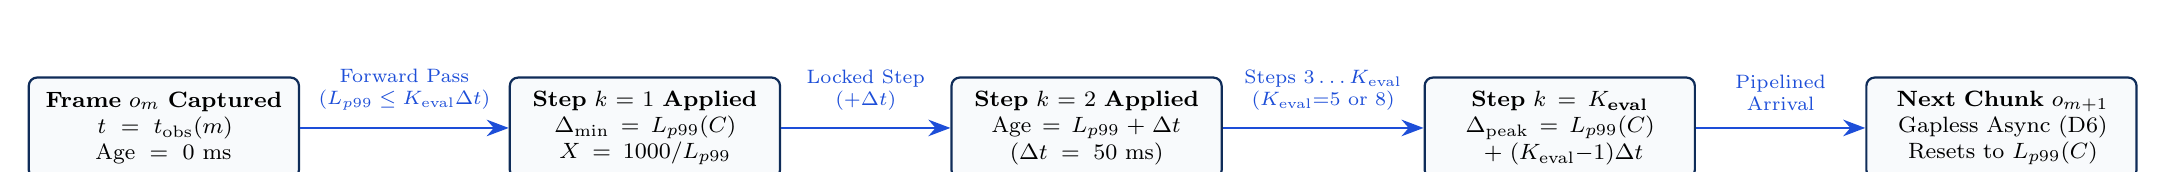
\begin{tikzpicture}[
    box/.style={rectangle, draw=navy, fill=boxbg, thick, rounded corners=3pt, minimum height=1.28cm, text width=3.15cm, inner sep=4pt, align=center, font=\footnotesize},
    arrow/.style={-{Stealth[length=2.8mm]}, thick, color=accent},
    alabel/.style={above=4pt, inner sep=2pt, font=\scriptsize, align=center}
]
\node[box] (O1) {\textbf{Frame $o_m$ Captured}\\$t = t_{\text{obs}}(m)$\\$\text{Age} = 0\text{ ms}$};
\node[box, right=2.65cm of O1] (A1) {\textbf{Step $k = 1$ Applied}\\$\Delta_{\min} = L_{p99}(C)$\\$X = 1000/L_{p99}$};
\node[box, right=2.15cm of A1] (A2) {\textbf{Step $k = 2$ Applied}\\$\text{Age} = L_{p99} + \Delta t$\\$(\Delta t = 50\text{ ms})$};
\node[box, right=2.55cm of A2] (AK) {\textbf{Step $k = K_{\text{eval}}$}\\$\Delta_{\text{peak}} = L_{p99}(C)$\\${}+ (K_{\text{eval}}{-}1)\Delta t$};
\node[box, right=2.15cm of AK] (AN) {\textbf{Next Chunk $o_{m+1}$}\\Gapless Async (D6)\\Resets to $L_{p99}(C)$};

\draw[arrow] (O1) -- node[alabel] {Forward Pass\\($L_{p99} \le K_{\text{eval}}\Delta t$)} (A1);
\draw[arrow] (A1) -- node[alabel] {Locked Step\\($+\Delta t$)} (A2);
\draw[arrow] (A2) -- node[alabel] {Steps $3\dots K_{\text{eval}}$\\($K_{\text{eval}}{=}5$ or $8$)} (AK);
\draw[arrow] (AK) -- node[alabel] {Pipelined\\Arrival} (AN);
\end{tikzpicture}%
}
\caption{Guaranteed interactivity $X(C) = 1000/L_{p99}(C)$ (D5) and co-reported Peak Age of Information $\Delta_{\text{peak}}(C, K_{\text{eval}})$ (D7) under locked horizon $K_{\text{eval}} \in \{5, 8\}$ and gapless asynchronous overlap (D6).}
\end{figure}

\subsection{Fleet Throughput and Hardware Normalizations}

\subsubsection{Steady-State Action and Prediction Throughput}
Across canonical grid $C \in \{1, 2, 4, 8, 16\}$ over the steady-state full-occupancy window $T_{\text{steady}}(C)$ (kept saturated via untimed keep-alive requests and verified by the $\le 15\%$ per-slot completion fairness fence), primary Fleet Throughput is:
\begin{equation}
    Y_{\text{VLA}}(C) = \frac{N_{\text{timed}}(C) \cdot K_{\text{eval}}}{T_{\text{steady}}(C)} \;\; [\text{Actions/s}], \qquad Y_{\text{WM}}(C) = \frac{N_{\text{timed}}(C)}{T_{\text{steady}}(C)} \;\; [\text{Predictions/s}]
\end{equation}
where each Track 2 rollout prediction generates $K_{\text{eval}} = 16$ future frames, and $20\text{ Actions/s}$ corresponds to one gapless $20\text{ Hz}$ VLA control stream.

\subsubsection{Power and Roofline Normalization Views}
From the identical run receipt, EmbodiedX computes the two plotted Season 1 leaderboard views (\texttt{Throughput vs.\ Interactivity} and \texttt{Efficiency vs.\ Interactivity}) plus two auxiliary schema normalizations (D5):

\begin{table}[ht!]
\centering
\footnotesize
\renewcommand{\arraystretch}{1.18}
\begin{tabularx}{\textwidth}{>{\bfseries\raggedright\arraybackslash}p{3.1cm} >{\centering\arraybackslash}p{3.9cm} >{\raggedright\arraybackslash}p{3.0cm} >{\raggedright\arraybackslash}X}
\toprule
\textbf{Y-Axis View} & \textbf{Physical Formula} & \textbf{Literature Basis} & \textbf{Role in EmbodiedX Season 1} \\
\midrule
1.\ Fleet Throughput\newline\normalfont\emph{(\texttt{Actions/s}, \texttt{Predictions/s})} & $\displaystyle\frac{Y_{\text{VLA}}(C)\text{ or }Y_{\text{WM}}(C)}{1\text{ chip}}$ & InferenceX \cite{Patel2025inferencemax}\newline MLPerf \cite{Reddi2020mlperf}\newline RobotPerf \cite{MayoralVilches2024robotperf} & Official \textbf{Real-Time Fleet Throughput} award metric over SLA-compliant discrete points in $\{1, 2, 4, 8, 16\}$ (D9). \\
\midrule
2.\ Green Efficiency\newline\normalfont\emph{(\texttt{Actions/J}, \texttt{Predictions/J})} & $\displaystyle\frac{Y(C)}{\bar{P}_{\text{board}}\text{ (W)}} = \frac{\text{Output}}{\text{Joule}}$ & MLPerf Power \cite{MLCommons2026power}\newline ML.ENERGY \cite{Chung2025mlenergy}\newline AI Energy Score \cite{Luccioni2025aienergy}\newline DeeR-VLA \cite{Yue2024deervla} & Official \textbf{Green Embodied Efficiency} award metric requiring \texttt{power\_provenance == "MEASURED"} via constant-cap \texttt{10 Hz NVML} board power on \texttt{NVIDIA L40S} (\texttt{-{}-assume-power-watts} rejected; \texttt{TPU v6e-1 = N/A}). \\
\midrule
3.\ Ref.\ Hourly Rate\newline\normalfont\emph{(Auxiliary \texttt{(Out/s)/(\$/hr)})} & $\displaystyle\frac{Y(C)}{\text{Ref.\ Rate (\$/hr)}}$ & InferenceX v2 \cite{Patel2026inferencexv2} & Auxiliary schema diagnostic against pinned on-demand cloud rates (\texttt{\textasciitilde\$0.88--\$1.15/hr} \texttt{L40S}, \texttt{\textasciitilde\$1.375/hr} \texttt{TPU v6e-1}). \\
\midrule
4.\ Roofline Iso-Views\newline\normalfont\emph{(Auxiliary \texttt{/100 TF}, \texttt{/TB/s})} & $\displaystyle\frac{Y(C)}{P_{\text{BF16}}/100}, \;\; \frac{Y(C)}{\text{BW}_{\text{peak}}}$ & Williams et al.\ \cite{Williams2009roofline} & Auxiliary Roofline efficiency metric against dense BF16 peak and memory BW ($362.05\text{ TF}$ / $864\text{ GB/s}$ \texttt{L40S}; $918\text{ TF}$ / $1{,}600\text{ GB/s}$ \texttt{TPU v6e-1}). \\
\bottomrule
\end{tabularx}
\caption{Primary plotted Season 1 leaderboard metrics (Views 1--2) and auxiliary Roofline/cost diagnostics (Views 3--4).}
\end{table}

\FloatBarrier
\section{Hardware Targets Verification Protocol and Season 1 Governance}

\subsection{Absolute Physical Units Over Relative Speedups}
Scoring relative speedup ($L_{\text{base}} / L_{\text{sub}}$) penalizes platforms with well-tuned reference compilers and prevents cross-platform comparison on a shared physical scale \cite{Patel2025inferencemax,Reddi2020mlperf}. EmbodiedX ranks submissions exclusively in absolute SI units (\texttt{Chunks/s}, \texttt{Predictions/s}, \texttt{Actions/s}, \texttt{Actions/J}, \texttt{Predictions/J}) with zero organizer-seeded vendor numbers.

\subsection{Standardized Season 1 Cloud Hardware Targets}
Every canonical workload ($2\text{B}$ to $3.3\text{B}$ parameters) fits comfortably on one device. Under \textbf{D8}, Season 1 standardizes strictly on two single-chip (\texttt{num\_devices == 1}, $\text{TP} = \text{PP} = \text{EP} = 1$) cloud accelerators at stock vendor TDP and clock limits so entries compete on device kernels, graph compilers, low-bit quantization, and request scheduling while organizers can re-run finalists on identical silicon:
\begin{enumerate}
    \item \textbf{Standard GPU (\texttt{nvidia\_l40s\_48gb}).} \textbf{\texttt{NVIDIA L40S}} (Ada Lovelace SM89, $48\text{ GB}$ GDDR6 at $864\text{ GB/s}$, $350\text{ W}$ board TDP, native FP8 Tensor Cores, $362.05\text{ TF}$ dense BF16, active \texttt{10 Hz NVML} board power telemetry). Available via Shadeform (\texttt{\textasciitilde\$0.88--\$1.15/hr}), AWS EC2 \texttt{g6e.xlarge}, or the NVIDIA Academic Grant Program.
    \item \textbf{Standard TPU (\texttt{tpu\_v6e\_1\_32gb}).} \textbf{\texttt{Google Cloud TPU v6e-1}} (Trillium single-chip slice, $32\text{ GB}$ HBM2e at $1{,}600\text{ GB/s}$, $918\text{ TF}$ dense BF16, $1{,}836\text{ TOPS}$ INT8/FP8; isolate multi-chip hosts via \path{TPU_CHIPS_PER_HOST_BOUNDS=1,1,1}, \path{TPU_HOST_BOUNDS=1,1,1}, and \path{TPU_VISIBLE_DEVICES=0}). Available via Google Cloud (\texttt{\textasciitilde\$1.375/hr}) or free through a renewable 30-day Google TPU Research Cloud (TRC) allocation.
\end{enumerate}
Additional single-chip and edge profiles remain in the hardware schema solely for local development and future onboard-edge seasons.

\subsection{Closed and Open Quality Gates and Scalar Award Categories}

Because crossing Pareto curves prevent a single total order, Season 1 crowns winners across three scalar categories inside each independent track pool (\texttt{Track 1A}, \texttt{Track 1B}, \texttt{Track 2}):

\begin{table}[ht!]
\centering
\footnotesize
\renewcommand{\arraystretch}{1.18}
\begin{tabularx}{\textwidth}{>{\bfseries\raggedright\arraybackslash}p{3.6cm} >{\raggedright\arraybackslash}p{6.2cm} >{\raggedright\arraybackslash}X}
\toprule
\textbf{Season 1 Award Category} & \textbf{Scalar Ranking Metric} & \textbf{Mandatory Admissibility Gate} \\
\midrule
1.\ Interactive Reactivity (\texttt{C = 1}) & Highest single-stream rate $1000 / L_{p99}(1)$ at $C = 1$ (lowest $C{=}1$ $p99$ latency, tie-broken by lowest $p50$ latency). & Unimodal tail $L_{p99}(1) / L_{p50}(1) \le 1.5$ plus full division quality gates ($\ge 100$ golden samples). \\
\midrule
2.\ Real-Time Fleet Throughput & Highest aggregate \texttt{Actions/s} (Track 1) or \texttt{Predictions/s} (Track 2) across canonical points $C \in \{1, 2, 4, 8, 16\}$. & Selected point must meet the gapless pooled $p99$ SLA ($\le 250$, $\le 400$, or $\le 1000\text{ ms}$) and $\le 15\%$ slot fairness fence. \\
\midrule
3.\ Green Embodied Efficiency & Highest hardware-measured \texttt{Actions/J} (Track 1) or \texttt{Predictions/J} (Track 2) over SLA-compliant grid points. & \texttt{power\_provenance == "MEASURED"} via constant-cap \texttt{10 Hz NVML} board power on \texttt{L40S} (\texttt{-{}-assume-power-watts} rejected; \texttt{TPU v6e-1 = N/A}). \\
\bottomrule
\end{tabularx}
\caption{Official EmbodiedX Season 1 scalar award categories per track. Exact scalar ties are broken by lower-step Real-Time Dominated Hypervolume wrt $(0.5 X_{\text{SLA}}, 0)$ over SLA-compliant discrete points in $\{1, 2, 4, 8, 16\}$ without curve interpolation.}
\end{table}

\subsection{Anti-Gaming Defenses and Two-Phase Commit-Reveal}
\begin{enumerate}
    \item \textbf{Eight-Gate Anti-Gaming Verifier (D4, D10).} Every bundle must pass eight automated checks: (i) single-chip isolation (\texttt{num\_devices == 1}) at stock TDP/clocks; (ii) canonical ordered grid $C \in \{1, 2, 4, 8, 16\}$ from $C = 1$ with monotonic OOM truncation only; (iii) locked $K_{\text{eval}}$ and real public traces from \path{HuggingFaceVLA/libero} and \path{lerobot/droid_100} at native wire payloads ($\ge 224\times 224$ RGB, zero synthetic sine waves); (iv) opaque random \texttt{UUIDv4} \texttt{session\_id}s plus dynamically seeded per-frame cryptographic $\pm 1/255$ \texttt{uint8} pixel micro-jitter banning hash lookup tables; (v) outlier fence $\max / p50 \le 4.0$, per-slot completion fairness skew $\le 15\%$, and $C{=}1$ tail unimodality $p99 / p50 \le 1.5$; (vi) $N = 3$ trial consistency ($\le 8\%$ pooled $p99$ spread across $N \ge 320$ VLA / $N \ge 200$ WM calls after \texttt{-{}-warmup >= 30} on the live model loop; lock SM clocks via \texttt{nvidia-smi -lgc} on the real workload only if boost trips variance); (vii) inline Golden-IO parity over \texttt{-{}-num-samples >= 100} real samples ($\text{CosSim} \ge 0.995$ + $\text{CVaR-1\%}$ on Track 1; $\text{SSIM} \ge 0.88$, $\text{PSNR} \ge 26.0\text{ dB}$, $\text{CVaR-1\%}(\text{SSIM}) \ge 0.80$, $\text{CVaR-1\%}(\text{PSNR}) \ge 22.0\text{ dB}$ on Track 2) and $\text{G4}$ sensitivity probes (\texttt{Closed}) or signed Stage-2 quality receipt (\texttt{Open}); and (viii) SHA-256 receipt integrity and constant-cap \texttt{MEASURED} NVML power verification (\texttt{torch.cuda.synchronize()}, \texttt{torch.tpu.synchronize()}, or \texttt{jax.block\_until\_ready()} before stopping request timers).
    \item \textbf{Two-Phase Commit-Reveal and Clean-Hardware Re-run.} In Phase 1, contestants package and verify public pull request bundles via \texttt{eeb prepare-commit-bundle} and \texttt{eeb verify-bundle -{}-strict}, submitting only \path{bundle_summary.json} and \path{submission_meta.json} carrying \path{recipe_commit_sha256}, the SHA-256 digest over canonical \path{reveal_manifest.json} (pinning immutable OCI container image \texttt{@sha256}, Hugging Face checkpoint commit SHA and shard SHA-256 digests, lockfile SHA-256, and CLI command). Within $24\text{ hours}$ after December 18, 2026 (\texttt{23:59 AoE}), shortlisted finalists (at most one finalist slot per lab or organization per track and division) privately supply their matching container and manifest. Final Official Season 1 Awards are ranked strictly by Phase-2 organizer clean-hardware re-runs on a private held-out split; agreement within $\pm 8\%$ of Phase 1 serves strictly as an anti-fraud disqualification gate. Confirmed Season 1 winners publish open recipes (\texttt{Verified Open Recipe}); rolling \texttt{2027+} entries support both open and \texttt{Proprietary / Audit-Only} attribution.
\end{enumerate}

\subsection{End-to-End Pipeline Validation Matrix and Season 1 Schedule}

All reference servers, public trace loaders, telemetry sidecars, and eight-gate validators were verified end-to-end on physical \texttt{NVIDIA L40S} and \texttt{Google Cloud TPU v6e-1} prior to release. Under Option A, Season 1 opens with $0$ seeded entries across all tracks (Table~\ref{tab:pipeline_matrix}).

\begin{table}[ht!]
\centering
\scriptsize
\setlength{\tabcolsep}{3.5pt}
\renewcommand{\arraystretch}{1.20}
\begin{tabularx}{\textwidth}{>{\raggedright\arraybackslash}p{3.65cm} >{\raggedright\arraybackslash}p{2.95cm} >{\raggedright\arraybackslash}p{4.05cm} >{\raggedright\arraybackslash}X c}
\toprule
\textbf{Track, Architecture, \& Checkpoint} & \textbf{Horizon, Traces, \& SLA} & \textbf{Division Quality Gates ($\ge 100$ Samples)} & \textbf{Validated Standard GPU (\texttt{L40S}) \& TPU (\texttt{v6e-1}) Stacks} & \textbf{Seeded} \\
\midrule
\textbf{Track 1A: $\pi_{0.5}$\text{-LIBERO}}\newline\texttt{lerobot/pi05\_libero\_}\newline\texttt{finetuned\_v044}\newline\texttt{@7152f13e34c6} & $H{=}10$, \textbf{locked $K_{\text{eval}}{=}5$}\newline\texttt{HuggingFaceVLA/libero}\newline Dual $224^2$ RGB, $10$ steps\newline$L_{p99} \le 250.0\text{ ms}$ ($\ge 4.0\text{ Chunks/s}$) & \textbf{Closed:} $\text{CosSim} \ge 0.995$ + $\text{CVaR-1\%}$\newline\textbf{Open:} Stage-2 \texttt{LIBERO-RT} within $-5.0\text{ pp}$ & \textbf{L40S:} \texttt{PyTorch} (\texttt{eager}/\texttt{compile}) + \texttt{10 Hz NVML}\newline\textbf{v6e-1:} \texttt{openpi JAX} (\texttt{jit}) \& \texttt{TorchTPU}; 8 gates verified & $0$ \\
\midrule
\textbf{Track 1B: \texttt{GR00T N1.7-3B}}\newline\texttt{nvidia/GR00T-N1.7-LIBERO}\newline(\texttt{libero\_10}, \texttt{@2ea293aa20ba}) & $H{=}16$, \textbf{locked $K_{\text{eval}}{=}8$}\newline\texttt{HuggingFaceVLA/libero}\newline Dual $256^2$ RGB, $16$ steps\newline$L_{p99} \le 400.0\text{ ms}$ ($\ge 2.5\text{ Chunks/s}$) & \textbf{Closed:} $\text{CosSim} \ge 0.995$ + $\text{CVaR-1\%}$\newline\textbf{Open:} Stage-2 \texttt{LIBERO-RT} within $-5.0\text{ pp}$ & \textbf{L40S:} \texttt{PyTorch} (\texttt{eager}/\texttt{compile}) + \texttt{10 Hz NVML}\newline\textbf{v6e-1:} \texttt{TorchTPU} (\texttt{eager}/\texttt{compile}); 8 gates verified & $0$ \\
\midrule
\textbf{Track 2: \texttt{Cosmos-Predict2.5-2B}}\newline\texttt{nvidia/Cosmos-Predict2.5-2B}\newline(\texttt{robot/action-cond}, \texttt{@85f8ae7bfe8f}) & \textbf{Locked $K_{\text{eval}}{=}16$} frames\newline\texttt{lerobot/droid\_100}\newline$256^2$ RGB, $10$ steps, $\text{CFG}{=}1$\newline$L_{p99} \le 1000\text{ ms}$ ($\ge 1.0\text{ Pred/s}$) & \textbf{Closed:} $\text{SSIM} \ge 0.88$, $\text{PSNR} \ge 26.0\text{ dB}$, $\text{CVaR-1\%} \ge 0.80 / 22.0\text{ dB}$\newline\textbf{Open:} + $\text{LPIPS} \le 0.12$, $\text{FVD} \le 120$, $\text{InvDyn} \ge 0.99$, $\tau \ge 0.80$ & \textbf{L40S:} \texttt{PyTorch} (\texttt{eager}/\texttt{compile}) + \texttt{10 Hz NVML}\newline\textbf{v6e-1:} \texttt{TorchTPU} \& \texttt{JAX} servers; 8 gates verified & $0$ \\
\bottomrule
\end{tabularx}
\caption{End-to-end validated pipeline and target platform specification matrix for EmbodiedX Season 1. Full 40-character Hugging Face commit SHAs appear in Section 1.1 (D2). Season 1 opens with $0$ pre-seeded vendor entries so community pull requests establish the founding Pareto frontier.}
\label{tab:pipeline_matrix}
\end{table}

\textbf{Season 1 Calendar and Winner Recognition.} Season 1 launches \textbf{October 30, 2026}. \textbf{Checkpoint 1 (November 10, 2026, 23:59 UTC)} freezes entries featured live on stage as Founding Frontier Leaders at the CoRL 2026 EEAI Workshop in Austin on \textbf{November 12, 2026}. \textbf{Checkpoint 2 (December 18, 2026, 23:59 AoE)} closes Season 1 awards (+24h finalist reveal; continuous rolling leaderboard in \texttt{2027+}). Verified Season 1 category winners receive \textbf{monetary prizes}, an official \textbf{CoRL 2026 EEAI Workshop Award Certificate}, \textbf{an invitation to apply for Google Cloud credits}, permanent verified leaderboard attribution, and an invitation to co-author the post-season \emph{EmbodiedX Season 1 Systems Report}.

\subsection{Planned Extensions Beyond Season 1}
Future seasons introduce planned additions (S2-1 and S2-2): (1) variable-horizon planning evaluated directly against Peak Age of Information $\Delta_{\text{peak}}(C, K)$ alongside sub-$100\text{ ms}$ frame-causal streaming world-model gates \cite{Chen2024diffusionforcing,Yin2025causvid,Huang2025selfforcing,Valevski2024gamengen,He2025matrixgame2}, and (2) dedicated onboard edge SoC divisions, multimodal omni policies (\texttt{Qwen3-Omni-30B-A3B} \cite{Qwen2025qwen3omni}), and physical robot evaluation arenas (\texttt{RoboArena} \cite{Atreya2025roboarena}).

\begingroup
\footnotesize
\raggedright
\bibliographystyle{unsrt}
\bibliography{references}
\endgroup

\end{document}
